\section{ Single Collector Algorithm (SCA)} 
\label{single}
We discuss here the single collection version of our algorithm; the multi-collection version will be discussed in Section \ref{multi}.
For the single collector version, we assume that every mutation in $G$ is serialized
and that the Adversary does not create or delete edges in $G$ during a \emph{collection process} (i.e. the sequence of messages and
state changes needed to determine the liveness of a node).
When the last strong edge to a node, $x$, in $G$ is deleted, but $\Gamma_{\rm in}(x)$ is not empty,
$x$ becomes an {\em initiator}. % A node is
%considered to be an initiator when it is uncertain about it's liveness, i.e. when
%it still has incoming edges, but loses its last strong edge.
The initiator node starts a set of graph traversals which we call phases:
{\em phantomization}, {\em recovery}, {\em building}, and {\em deletion}. We classify the latter three
phases as {\em correction} phases.
%All phases will run in the order listed on any given node, except that
%recovery and deletion will only occur in certain situations.
Fig.~\ref{fig:state} provides a flow diagram of the phases of an initiator. 
\begin{figure}
\centering
%\begin{center}
\scalebox{0.6}[0.6]{% Graphic for TeX using PGF
% Title: C:\Users\Hari\Pictures\Diagram2.dia
% Creator: Dia v0.97.2
% CreationDate: Wed May 11 10:06:32 2016
% For: Hari
% \usepackage{tikz}
% The following commands are not supported in PSTricks at present
% We define them conditionally, so when they are implemented,
% this pgf file will use them.
\ifx\du\undefined
  \newlength{\du}
\fi
\setlength{\du}{15\unitlength}
\begin{tikzpicture}
\pgftransformxscale{1.000000}
\pgftransformyscale{-1.000000}
\definecolor{dialinecolor}{rgb}{0.000000, 0.000000, 0.000000}
\pgfsetstrokecolor{dialinecolor}
\definecolor{dialinecolor}{rgb}{1.000000, 1.000000, 1.000000}
\pgfsetfillcolor{dialinecolor}
\definecolor{dialinecolor}{rgb}{1.000000, 1.000000, 1.000000}
\pgfsetfillcolor{dialinecolor}
\pgfpathellipse{\pgfpoint{14.956636\du}{4.226682\du}}{\pgfpoint{3.143364\du}{0\du}}{\pgfpoint{0\du}{1.876682\du}}
\pgfusepath{fill}
\pgfsetlinewidth{0.100000\du}
\pgfsetdash{}{0pt}
\pgfsetdash{}{0pt}
\pgfsetmiterjoin
\definecolor{dialinecolor}{rgb}{0.000000, 0.000000, 0.000000}
\pgfsetstrokecolor{dialinecolor}
\pgfpathellipse{\pgfpoint{14.956636\du}{4.226682\du}}{\pgfpoint{3.143364\du}{0\du}}{\pgfpoint{0\du}{1.876682\du}}
\pgfusepath{stroke}
% setfont left to latex
\definecolor{dialinecolor}{rgb}{0.000000, 0.000000, 0.000000}
\pgfsetstrokecolor{dialinecolor}
\node at (14.956636\du,4.466682\du){};
% setfont left to latex
\definecolor{dialinecolor}{rgb}{0.000000, 0.000000, 0.000000}
\pgfsetstrokecolor{dialinecolor}
\node[anchor=west] at (12.441636\du,4.351682\du){\textbf{Phantomization}};
\definecolor{dialinecolor}{rgb}{1.000000, 1.000000, 1.000000}
\pgfsetfillcolor{dialinecolor}
\pgfpathellipse{\pgfpoint{18.668364\du}{10.980046\du}}{\pgfpoint{2.178364\du}{0\du}}{\pgfpoint{0\du}{1.576682\du}}
\pgfusepath{fill}
\pgfsetlinewidth{0.100000\du}
\pgfsetdash{}{0pt}
\pgfsetdash{}{0pt}
\pgfsetmiterjoin
\definecolor{dialinecolor}{rgb}{0.000000, 0.000000, 0.000000}
\pgfsetstrokecolor{dialinecolor}
\pgfpathellipse{\pgfpoint{18.668364\du}{10.980046\du}}{\pgfpoint{2.178364\du}{0\du}}{\pgfpoint{0\du}{1.576682\du}}
\pgfusepath{stroke}
% setfont left to latex
\definecolor{dialinecolor}{rgb}{0.000000, 0.000000, 0.000000}
\pgfsetstrokecolor{dialinecolor}
\node at (18.668364\du,11.220046\du){\textbf{Recovery}};
% setfont left to latex
\definecolor{dialinecolor}{rgb}{0.000000, 0.000000, 0.000000}
\pgfsetstrokecolor{dialinecolor}
\node[anchor=west] at (9.818364\du,11.005046\du){};
\definecolor{dialinecolor}{rgb}{1.000000, 1.000000, 1.000000}
\pgfsetfillcolor{dialinecolor}
\pgfpathellipse{\pgfpoint{10.268364\du}{18.130046\du}}{\pgfpoint{2.178364\du}{0\du}}{\pgfpoint{0\du}{1.576682\du}}
\pgfusepath{fill}
\pgfsetlinewidth{0.100000\du}
\pgfsetdash{}{0pt}
\pgfsetdash{}{0pt}
\pgfsetmiterjoin
\definecolor{dialinecolor}{rgb}{0.000000, 0.000000, 0.000000}
\pgfsetstrokecolor{dialinecolor}
\pgfpathellipse{\pgfpoint{10.268364\du}{18.130046\du}}{\pgfpoint{2.178364\du}{0\du}}{\pgfpoint{0\du}{1.576682\du}}
\pgfusepath{stroke}
% setfont left to latex
\definecolor{dialinecolor}{rgb}{0.000000, 0.000000, 0.000000}
\pgfsetstrokecolor{dialinecolor}
\node at (10.268364\du,18.370046\du){\textbf{Build}};
\definecolor{dialinecolor}{rgb}{1.000000, 1.000000, 1.000000}
\pgfsetfillcolor{dialinecolor}
\pgfpathellipse{\pgfpoint{25.768364\du}{18.380046\du}}{\pgfpoint{2.579644\du}{0\du}}{\pgfpoint{0\du}{1.867125\du}}
\pgfusepath{fill}
\pgfsetlinewidth{0.100000\du}
\pgfsetdash{}{0pt}
\pgfsetdash{}{0pt}
\pgfsetmiterjoin
\definecolor{dialinecolor}{rgb}{0.000000, 0.000000, 0.000000}
\pgfsetstrokecolor{dialinecolor}
\pgfpathellipse{\pgfpoint{25.768364\du}{18.380046\du}}{\pgfpoint{2.579644\du}{0\du}}{\pgfpoint{0\du}{1.867125\du}}
\pgfusepath{stroke}
% setfont left to latex
\definecolor{dialinecolor}{rgb}{0.000000, 0.000000, 0.000000}
\pgfsetstrokecolor{dialinecolor}
\node at (25.768364\du,18.620046\du){\textbf{Deletion}};
\pgfsetlinewidth{0.100000\du}
\pgfsetdash{}{0pt}
\pgfsetdash{}{0pt}
\pgfsetbuttcap
{
\definecolor{dialinecolor}{rgb}{0.000000, 0.000000, 0.000000}
\pgfsetfillcolor{dialinecolor}
% was here!!!
\pgfsetarrowsstart{stealth}
\definecolor{dialinecolor}{rgb}{0.000000, 0.000000, 0.000000}
\pgfsetstrokecolor{dialinecolor}
\pgfpathmoveto{\pgfpoint{19.896530\du}{9.625575\du}}
\pgfpatharc{29}{-64}{3.869885\du and 3.869885\du}
\pgfusepath{stroke}
}
\pgfsetlinewidth{0.100000\du}
\pgfsetdash{}{0pt}
\pgfsetdash{}{0pt}
\pgfsetbuttcap
{
\definecolor{dialinecolor}{rgb}{0.000000, 0.000000, 0.000000}
\pgfsetfillcolor{dialinecolor}
% was here!!!
\pgfsetarrowsend{stealth}
\definecolor{dialinecolor}{rgb}{0.000000, 0.000000, 0.000000}
\pgfsetstrokecolor{dialinecolor}
\pgfpathmoveto{\pgfpoint{13.834722\du}{6.026196\du}}
\pgfpatharc{210}{187}{27.410428\du and 27.410428\du}
\pgfusepath{stroke}
}
\pgfsetlinewidth{0.100000\du}
\pgfsetdash{}{0pt}
\pgfsetdash{}{0pt}
\pgfsetbuttcap
{
\definecolor{dialinecolor}{rgb}{0.000000, 0.000000, 0.000000}
\pgfsetfillcolor{dialinecolor}
% was here!!!
\pgfsetarrowsend{stealth}
\definecolor{dialinecolor}{rgb}{0.000000, 0.000000, 0.000000}
\pgfsetstrokecolor{dialinecolor}
\pgfpathmoveto{\pgfpoint{16.759366\du}{11.816219\du}}
\pgfpatharc{243}{216}{15.710313\du and 15.710313\du}
\pgfusepath{stroke}
}
\pgfsetlinewidth{0.100000\du}
\pgfsetdash{}{0pt}
\pgfsetdash{}{0pt}
\pgfsetbuttcap
{
\definecolor{dialinecolor}{rgb}{0.000000, 0.000000, 0.000000}
\pgfsetfillcolor{dialinecolor}
% was here!!!
\pgfsetarrowsstart{stealth}
\definecolor{dialinecolor}{rgb}{0.000000, 0.000000, 0.000000}
\pgfsetstrokecolor{dialinecolor}
\pgfpathmoveto{\pgfpoint{25.439190\du}{16.478320\du}}
\pgfpatharc{344}{292}{7.799925\du and 7.799925\du}
\pgfusepath{stroke}
}
% setfont left to latex
\definecolor{dialinecolor}{rgb}{0.000000, 0.000000, 0.000000}
\pgfsetstrokecolor{dialinecolor}
\node[anchor=west] at (4.370000\du,7.853364\du){\textbf{If Build Set is non-empty}};
% setfont left to latex
\definecolor{dialinecolor}{rgb}{0.000000, 0.000000, 0.000000}
\pgfsetstrokecolor{dialinecolor}
\node[anchor=west] at (19.920000\du,5.603364\du){\textbf{If Build Set is empty}};
% setfont left to latex
\definecolor{dialinecolor}{rgb}{0.000000, 0.000000, 0.000000}
\pgfsetstrokecolor{dialinecolor}
\node[anchor=west] at (13.170000\du,15.503364\du){\textbf{If Recovery set is non-empty}};
% setfont left to latex
\definecolor{dialinecolor}{rgb}{0.000000, 0.000000, 0.000000}
\pgfsetstrokecolor{dialinecolor}
\node[anchor=west] at (22.920000\du,12.053364\du){\textbf{If Recovery set is emtpy}};
\end{tikzpicture}
}
\caption{The above figure depicts the phase transitions performed by initiator in the algorithm.
}
\label{fig:state}
%\end{center}

\end{figure}



\paragraph{}

%According to %

%\cref{def:path,def:strongpath,def:nonstrongpath,def:related,def:dep,def:puredep,def:sup,def:indep,def:build,def:rec,def:aff},
As illustrated in Fig.~\ref{fig:completeabstract}, a node $A\in G$ is dead if and only if its supporting set
is empty. If $A$ is discovered to be dead, then its purely dependent set is also
dead. % Our algorithm searches for $C'$ (which contains nodes that have paths
%leading to and coming from $A$), and detmines whether $D'$ (which only contains nodes with paths
%leading to $A$) is present.
%Because of our algorithm only traverses edges from the initiator, the nodes in
%will not be known to $A$, but $A$ will still be able to determine if build set is empty.
%Note that some nodes in the build set are outside the affected set (i.e. the nodes in $F$).
Even when the supporting set does
not intersect the affected set (i.e. when $C'$, $D'$ and $E'$ are empty), and thus
nodes in the build set do not receive any messages, our algorithm will still detect whether the
supporting set is empty. Appendix ~\ref{singlealgo} contains the detailed pseudocode of the single collector algorithm. We describe the phantomization and correction (recovery, building, and deletion) phases separately below.

\subsection{Phantomization Phase}
For a node of $G$ to become a phantom node, the node must
(1) have just lost its last strong edge, and
(2) not already be a phantom node.
Each node has a flag that identifies it as a phantom node.
The initiator node is, therefore, always a phantom node, and
phantomization always begins with the initiator.
When a node $w$ becomes a phantom node, it notifies
$\Gamma_{\rm out}(w)$ of this fact with {\em phantomize} messages. From that point on, all the outgoing edges from $w$ will
be considered to be {\em phantom edges}, i.e. neither strong nor weak but a transient and
indeterminate state. If a node, $u$, in $\Gamma_{\rm out}(w)$ loses its last strong edge
as a result of receiving a {\em phantomize} message, $u$ also becomes phantom node, %(i.e. if $u$ has any weak
%edges, it sets its $weight$ to $max_weight+1$, sends the phantomize message to $\Gamma_{\rm out}(u)$,
%and marks itself phantomized)
but not an initiator.
Phantomization will thus
mark all nodes in the dependent set.
%The set of nodes marked by the phantomization are called phantomized
All the nodes that receive the phantomize message are called {\em affected nodes}.
%The set $D$ will not but phantomized, but it is affected since nodes in this
%set will have some of their edges phantomized.
%Phantomization adjusts the edge labels of the affected nodes.

%\begin{lemma}[No Phantomization]
%If a strong path from the root to a node, $x$, exists, then $x$ will not
%phantomize.
%\label{lem:nophantomization}
%\end{lemma}
%\begin{proofs}
%A node will not phantomize unless it loses its last strong reference.
%\end{proofs}

%\begin{lemma}[Phantomization]
%If no strong path from the root to a node, $x$, exists, and $x$ is in the
%dependent set of an initiator node, then $x$ will phantomize.
%\label{lem:nophantomization}
%\end{lemma}
%\begin{proofs}
%\end{proofs}

Since the algorithm proceeds in phases, we need to wait for phantomization to complete before recovery or building can begin. For this reason,
for every \emph{phantomize} message sent from a node, $x$, to a node, $y$, a {\em return} message must be received by $x$ from $y$ . If
$y$ does not phantomize as a result of receiving the message from $x$, the {\em return}
is sent back to $x$ immediately. If the {\em phantomize} message causes $y$ to phantomize,
then $y$ waits until it has received {\em return} back from all nodes in $\Gamma_{\rm out}(y)$ before
replying to $x$ with {\em return}.
For this purpose, each phantom node maintains %an information in memory about
a single backward-pointing edge and a counter to track the number of {\em return} messages it is
waiting for. While $y$ is waiting for {\em return} messages, it is said to be {\em phantomizing}. Once
all \emph{return} messages are received, the phantom node is said to be {\em phantomized}.

%During the correction
%phase, our algorithm detects whether the sets $C'$ or $D'$ are non-empty. If they non-empty,
%it readjusts the edge labels (weights) in the graph and clears the phantomization bit.
% If no such set exist, then
%our algorithm tries to readjust the labels in $C$ and $C'$ and delete $A$ , $B$
%and $B'$.
%Correction is a three step phase. It involves searching
%for $C'$ and $D'$, readjusting the labels if necessary, and also deleting $A$,
%$B$, and $B'$ nodes in the graph if $C' \cap D'$ is empty.

%\subsubsection{Phantomization}

Phantomization is, therefore, essentially, a breadth-first search
rooted at the initiator.
%It will identify the affected nodes, i.e. the subset of the dependent and independent sets of nodes
%that are reachable from initiator.
%The process uses a message
%called \emph{phantomize} to find affected nodes.
The traversal contains two steps. In the forward
step, messages originate from the initiator and propagate to the affected nodes.
After they reach all the affected nodes,
\emph{return} messages will propagate backward to the initiator.
The reverse step is
a simple termination detection process which uses
a spanning tree in the subgraph comprised of the affected nodes (i.e., the single
backward-pointing edge forms the spanning tree).
%Each node will
%contain a parent pointer that is set when the node receives the first
%\emph{phantomize} message. During reverse step, each node will send \emph{return}
%message to the parent.

The edges of any phantom node are said to be \emph{phantom edges}.
%To distinguish the nodes that are part of the
%dependent set, our algorithm uses a flag for each node called \emph{phantomized}
%that identifies all outgoing edges of phantomized nodes as phantom edges. % A node and its
%outgoing edges are said to be
%phantomized if the \emph{phantomized flag} is set to true.
%On receiving a \emph{phantomize message}, based on the node's state, a node may send
%phantomize message to outneighbors. When a node sends phantomize message to
%outneighbors, it is said to be \emph{phantomized} and marks the propogation of
%phantomize message by setting the \emph{phantomized} flag. When a \emph{phantomize}
%message is sent from a node to another, the edge between them is said to converted to
%phantom. In addition to
Each node has a counter for its incoming phantom edges
(in addition to its strong and weak counter). Every node in the affected subgraph
will have a positive phantom count at the end of the phantomization phase. The initiator then enters to the correction phase. 
%This counter counts the number of incoming
%phantom edges and also, node updates the loss of strong and weak edges in their
%appropriate counter when the edges are converted into phantom.

%We mentioned that a node will send phantomize message to outneighbors based on
%certain conditions.

In addition to sending phantomize messages to its $\outneighbors$, when a node satisfies the
above conditions and contains only weak incoming edges, the node converts all the weak
incoming edges into strong incoming edges. %then sends the \emph{phantomize message} to its $\outneighbors$.
The process of converting all the weak incoming edges into strong
edges is called \emph{toggling}. Toggling is achieved by updating the weight
of the node to the maximum weight of its in-neighbors plus one ($weight \leftarrow \maxweight+1$).
%Every message sent
%in our algorithm always contain the weight of the node sending the message. At any
%point in time, all the nodes are aware of the maximum in-neighbor's weight.

%As we discussed above, the forward step
%along with finding the affected nodes, it also creates a spanning tree with parent
%pointer set for all the affected nodes to send the \emph{return} message back to
%initiator eventually. Return messages are also send to non-parent nodes /
%\emph{phantomize} message sender in certain cases as mentioned below:
%\begin{enumerate}
%\item If a node receives a phatonmize message and  is already phantomized after
%updating counters, it sends \emph{return} message to sender.
%\item If a node receives a phantomize message and  contains strong incoming edges
%after updating counters, it sends \emph{return} message to sender.
%\end{enumerate}

%When a node receives return messages from all the outneighbors,
%the node sends the return message to parent. When initiator receives return
%messages from children, the phantomization is said to be completed.
%\begin{definition}{Round:}
%We define rounds in the manner used by the $\mathcal{CONGEST}$ asynchronous model. A
%computation initiated by a node, $x$, is said to be in the $rth$ round if
%all $r$-neighborhoods of $x$ received the message.
%\end{definition}
\begin{comment}
\begin{lemma}[Time Complexity]
Phantomization finishes in O(Rad(i,$G_{a}$)) time, where $G_{a}$ is the graph
induced by affected nodes, i is the initiator, and Rad(i, $G_{a}$) is the radius
of the graph from from i.
\label{TimeP}
\end{lemma}
\begin{proofs}
%In r rounds, we assume at least r neighborhoods of i received the \emph{phantomize}
%message. The \emph{phantomize} message must reach all nodes in the $G_{a}$ from i.
In each time step, \emph{phantomization} spreads to the $\outneighbors$ of the previously
affected nodes, increasing the radius of the graph of phantomized nodes by 1.
In O(Rad(i,$G_{a}$)) time, all the nodes in $G_{a}$ receive
a \emph{phantomize} message, since all the nodes in $G_{a}$ are at distance less than
or equal to Rad(i,$G_{a}$) from i. In the reverse step, the same argument can be
applied backward.
%In r time, the $( Rad(i,G_{a}) - r) ^{th}$ neighborhood of i
%receives the \emph{return} messages.
So phantomization completes in O(Rad(i,$G_{a}$) time.
\end{proofs}

\begin{lemma}[Communication Complexity]
Phantomization uses O($E_{a}$) messages, where $E_{a}$ is the number of edges
in the graph induced by affected nodes.
\label{CCP}
\end{lemma}
\begin{proofs}
In the forward step of the algorithm, all the nodes in the dependent set send the
\emph{phantomize} message to their $\outneighbors$, and each node can do this at most
once (after which the \emph{phantomized} flag is set).
So the forward step of the algorithm uses only
O($E_{a}$) messages. In the reverse step, the \emph{return} messages are sent
backward along the edges of the spanning tree. So the reverse step sends O($V_{a}$)
messages, where $V_{a}$ is the number of nodes in the affected subgraph.
So Phantomization uses O($E_{a}$) messages.
\end{proofs}

\begin{lemma}[Message size Complexity]
Phantomization sends messages of O(log(n)) size, where n is the total number of nodes
in the graph.
\label{MSCP}
\end{lemma}
\begin{proofs}
The \emph{phantomize} messages have to hold a value at least as large as the count of nodes in the system
which are O(log(n)) size. Apart from the ids, the message also contains the weight of
node which is constant in size. In the return message, our algorithm only uses the id
of the sender and receiver. So all our messages in the phantomization are of
O(log(n)) size.
\end{proofs}

\end{comment}

\subsection{Correction Phase}

%Correction includes computing the
%supporting set, readjusting the labels and weights of the supporting set
%exists, and deleting a set of nodes if the supporting set is empty.
%After
%phantomization is complete,
The initiator starts either the \emph{recovery} or \emph{building} phase depending on the build set. 
%the initiator checks to see whether the build set is empty (i.e. if the initiator
%has strong edges).
If the build set is empty, the initiator enters the recovery phase; if it is
not empty, it enters the building phase.
In the building phase, the affected subgraph is traversed, phantom edges are
converted to strong and weak edges, and the weights of the nodes are adjusted.
%If the initiator finds out that the build
%set is empty (i.e. if the initiator has no incoming strong edges), then the direct building of the
%affected subgraph is not possible. The next phase is \emph{recovery}.
In the recovery phase, the affected subgraph is traced until the recovery set is found (i.e. phantom nodes
that have strong incoming edges). If and when this set is found, building phase begins. If not
the initiator deletes itself and all the purely
dependent nodes. We describe each phase in detail below.  

\paragraph{Building Phase:}
If the initiator has any strong incoming edges after the phantomization phase, then
the build set is not empty. In response, the initiator updates its phase to \emph{building}
and sends \emph{build} messages to
its $\outneighbors$, which convert phantom edges to strong or weak edges.

If a node, $y$, sends a \emph{build} message to a node, $x$, that is phantom node, the
$\maxweight$ of $x$ is set to the weight of $y$ ($x.\maxweight \leftarrow y.weight$),
and the weight of $x$ is set to the weight of $y$ plus one ($x.weight \leftarrow
y.weight+1$).  The node $x$ then
decrements the phantom count, increments the strong count, and
propagates the \emph{build} message to its $\outneighbors$.

If a node, $y$, sends a \emph{build} message to a node, $x$, that is not phantom node, it
updates the $\maxweight$ of $x$ if necessary, decrements
the phantom count and increments either the strong or the weak count, depending
on whether $y.weight < x.weight$. % of $y$ is less than the $weight$ of $x$ or not.

After a node, $x$, builds its last phantom edge and replies to its parent in the spanning tree with
\emph{return} (if it is the initiator node, it does not do this),
$x$ is then returned to a
\emph{healthy} state (i.e. all flags set to false,
etc.).

%(or
%possibly a phantom edge to a weak edge if other strong edges are already
%present on the receiving node).


%The phantomization, building, and recovery
%phases of the algorithm each contain two steps, forward and reverse.  In
%building, the forward step converts the phantom edges to strong or weak edges.
%In all cases, the reverse step detects the termination of the phase.

\begin{lemma}[Not Phantomized]
After phantomization, nodes in the build set are not phantom nodes.
\label{lem:nophan}
\end{lemma}
\begin{proof}
Appendix ~\ref{proofapp} contains the proof.
\end{proof}

\begin{lemma}[Build set]
After phantomization, if the initiator has strong incoming edges, then the
initiator is not dead.
\label{lem:buildset}
%nodes that are the source of those
%strong edges form the build set.
\end{lemma}
\begin{proof}
Appendix ~\ref{proofapp} contains the proof.
\end{proof}

%All nodes that are not already building that
%receive a build message change their status to building, and propagate the message along
%their outgoing edges.
%A node that sent a \emph{return} message in the building state will become a
%healthy node with no markings (i.e. no collection id, phantom count, etc.), thus removing itself from the phantomized subgraph and the collection process.

Like the phantomization phase, the building phase has a forward and reverse step and creates a spanning tree by resetting the parent attribute of the node in the same way as phantomization (i.e. when it
receives the first \emph{build} message). When all its $\outneighbors$ reply with \emph{return}, it sends \emph{return} to its parent.
A node that receives a \emph{build} message, but is already building, builds the phantom edge and sends the \emph{return} message to the sender.
%When a node receives a \emph{build} message in the
%forward step, the node converts the incoming phantom edge into strong or weak
%and  propagates under following condition:
%if the node finished the reverse step of phantomization or correction phase and it is not
%healthy node, then node converts the phantom edge to strong edge and
%propagates the \emph{build} message to out-neighbors. Otherwise, the node sends
%\emph{return} message to the sender.


%Forward step adjusts the weight of the node to have a strong path, if there is no
%strong path exist for the node. The idea behind creating the strong path is if a node
%receives a \emph{build} message from a node, the sender of \emph{build} message has a
%strong path already and to create a strong path, the node simply adjusts the weight of
%the node to higher than the weight of the \emph{build} message sender. Every message
%in the algorithm contains the weight of the node. If the node already has a strong path,
%then node simply updates the max-weight of the node and interprets the type of the edge
%from the sender's weight. After the build message is processed, the counters are updated
%to reflect the updated edges. Apart from the counters, the phatnomized flag is reset
%upon propagating the build message to out-neighbors. The node changes the state to
%building upon propagating the build message. A node sends the return message in the building
%step only if a node receives a build message when it is in healthy state or forward step in
%any part of the correction phase or no out-neighbors.

%At the end of the build process, the return messages are transmitted back and the initiator
%terminates the build process. The build process makes all the affected nodes become healthy
%and no node will have any marking or any non-zero counts in the phantom counter. If the
%build set is empty, the recovery process begins. Lemma \ref{TimeP},\ref{CCP}, and \ref{MSCP}
%holds true for the building process too as the building process is very similar to the
%phantomization except the algorithm removes the labels in the affected subgraph rather than
%the marking the nodes.

%\subsubsection*{Recovering}
\paragraph{Recovery Phase:}
%When the build set is empty, then the \emph{recovery phase} of the algorithm proceeds.
Recovery is the search for the recovery set. If found, a build of the subgraph of
nodes that are reachable from recovery set of nodes will begin. It is possible that the
recovery phase can build edges to the initiator and thereby rebuild the entire
affected set.


\begin{lemma}[Phantomized]
After phantomization, nodes in the recovery set are phantom nodes.
\label{lem:phant}
\end{lemma}
\begin{proof}
Appendix ~\ref{proofapp} contains the proof.
\end{proof}

\begin{lemma}[Recovery set]
After phantomization,
if a phantom node contains at least one strong incoming edge,
it belongs to the recovery set.
\label{lema:recoveryset}
\end{lemma}
\begin{proof}
Appendix ~\ref{proofapp} contains the proof.
\end{proof}

After the phantomization phase is complete, all phantom nodes that contain strong
incoming edges are members of the recovery set.  Once a set of phantomized nodes
with strong edges are detected, the building process described above can begin
from those nodes.

%Recovery uses the \emph{recovery} message to distinguish the process of
%searching for the recovery set.
When a phantom node with zero strong count %in the recovery set
%(i.e. a phantom node that has strong incoming edges)
receives a \emph{recovery}
message
it simply updates its state to \emph{recovering} and
propagates the \emph{recovery} message to $\outneighbors$. As in phantomization, when it receives all
\emph{return} messages back, it changes its state to \emph{recovered}. Also, as in phantomization
and building, a spanning tree and \emph{return} messages will be used to track
the progress of recovery.
If a node receives a \emph{recovery} message and that node has incoming
strong edges, it immediately starts building instead of recovering.

Note that it is possible for a build message to reach a node, $x$, that is still in
the forward step of the recovery process.  To accommodate this, when $x$
receives all its \emph{return} messages back from $\Gamma_{\rm out}(x)$,
$x$ checks to see if it now belongs to the recovery set (i.e. if it has positive strong
count). If it still does not belong to the recovery set, then the return
message is sent back to the parent as usual. If it is part of recovery set, the
node starts the build process. Any building node that sends the
\emph{return} message to its parent is not part of the phantomized subgraph and becomes
healthy, i.e. it is no longer part of any collection process.

%only if a node that is already in the recovering state
%received a recovery message or it is healthy node or no out-neighbors exist to
%propagate the message. If a node in recovering state received all the return
%messages and it does not have any strong incoming edge, it changes itself into
%recovered state and sends the return message to parent. The check to have
%strong incoming edge is to make sure that the node does not belong to recovery
%set as a result of any build process initiated by other nodes. If it belong to
%the recovery set, the node initiates the build process and at the end of the
%build process, it sends return message to the parent.





%\subsubsection*{Deletion}
\paragraph{Deletion Phase:}
%Deletion of edges by the Adversary is different from deletion of edges by a collector. Collectors
%use different type of message to delete the edges.
If the recovery phase finishes and the initiator, $x$, still has no incoming strong edge, it issues
\emph{plague delete} messages to $\Gamma_{\rm out}(x)$. %along its outgoing edges.
As the name suggests, this message is contagious and deadly. Any node receiving it decrements
its phantom count by one and (if the recipient has no incoming strong edges)
it sends the \emph{plague delete} message along its outgoing edges.
Once a node has no edges (i.e. phantom, strong, and weak count are zero), it is deleted.
Unlike the other phases, there is no \emph{return} message for the \emph{plague delete} message.
%traversal. A node will not be deleted until all its incoming edges are deleted.
%Plague delete
%does not have two step process. It is single step process. Once the initiator decided it cannot
%build on the return message from the out-neighbors, it initiates the plague delete message.
%The plague delete message deletes all the out-going edges which in turn decreases the counters of
%the out-neighbors. If the neighbors are part of the recovered nodes in the recovery, they
%propagate plague delete messages to out-neighbors. A node will stop plague delete only if it has
%any strong incoming edges. A node will delete itself when a node does not have any out-going
%neighbors and no incoming edges. Again as we reasoned the recovery part, plague delete is sent
%for each edge and each edge is being deleted as plague delete is sent.
\begin{comment}
\begin{lemma}[Plague Delete]
There are O($E_{a}$) plague delete messages sent and they require O(Rad(i,$G_{a}$)) time to finish the plague deletion.
\end{lemma}
\begin{proof}
In every forward step of the plague delete, all outgoing edges are consumed, and the message spreads outward by
a radius of 1. Therefore, in O(Rad(i,$G_{a}$)) time it will spread to the entire subgraph.
\end{proof}

\begin{lemma}
All nodes that have a strong count at the end of phantomization are live.
\end{lemma}
\begin{proof}
Assume there exists a node, $x$, that is dead, but has a strong count. If the
node is dead, it must either (1) be the initiator, or (2) belong to the purely dependent
set. If the $x$ is an initiator, then the strong count comes from the
build set, but there exists a path from $R$ to all nodes in the build set. So option (1)
contradicts our assumption. After
phantomization, all of the nodes in the purely dependent set will only have incoming
phantom edges. So option (2) also contradicts our
assumption.
\end{proof}
\end{comment}
\begin{lemma}[Time Complexity]
SCA finishes in O(Rad(i,$G_{a}$)) time, where $G_{a}$ is the graph
induced by affected nodes, i is the initiator, and Rad(i, $G_{a}$) is the radius
of the graph from from i.
\label{TimeC}
\end{lemma}
\begin{proof}
Appendix ~\ref{proofapp} contains the proof.
\end{proof}

\begin{observation}
SCA finishes in O($E_a$) time, since Rad(i, $G_{a}$) can be O($E_a$).
\end{observation}
\begin{lemma}[Communication Complexity]
SCA sends O($E_{a}$) messages, where $E_{a}$ is the number of edges
in the graph induced by affected nodes.
\label{CCC}
\end{lemma}
\begin{proof}
Appendix ~\ref{proofapp} contains the proof.
\end{proof}


\begin{lemma}[Message Size Complexity]
SCA sends messages of O(log(n)) size, where n is the total number of nodes
in the graph.
\label{MSCP}
\end{lemma}
\begin{proof}
Appendix ~\ref{proofapp} contains the proof.
\end{proof}


\begin{theorem}
All dead nodes will be deleted at the end of the correction phases.
\label{pro:livenesss}
\end{theorem}
\begin{proof}
Appendix ~\ref{proofapp} contains the proof.
\end{proof}

\begin{theorem}
No live node will be deleted at the end of the correction phases.
\label{pro:safetys}
\end{theorem}

\begin{proof}
Appendix ~\ref{proofapp} contains the proof.


\end{proof}

\begin{comment}
\begin{center}
\begin{figure}
\centering
\includegraphics[scale = 0.25]{figs/vennpng}
\caption{ Venn diagram of relationship among sets used by algorithm.
}
\label{fig:vennpng}
\end{figure}
\end{center}

\def \setA{ (0,0) circle (1cm) }
\def \setB{ (1.5,0) circle (1cm) }
\def \setC{ (3.0,0) circle (1cm) }
\def \setU{ (-2, -1.5) rectangle (5.5, 2.0) }
\begin{center}
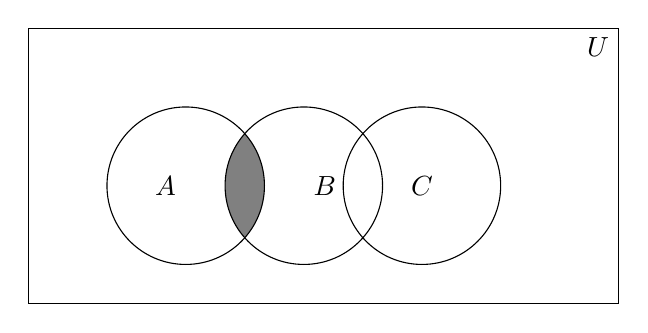
\begin{tikzpicture}
\draw \setU node[below left]{$U$};
\begin{scope}
\clip \setA;
\fill[gray] \setB;
\end{scope}
\begin{scope}
\clip \setA;
\clip \setB;
\fill[white] \setC;
\end{scope}
\draw \setA node[left] {$A$};
\draw \setB node[right] {$B$};
\draw \setC node {$C$};
\end{tikzpicture}
\end{center}
\end{comment}
